\section{Processi supporto}
<<<<<<< HEAD
=======

>>>>>>> develop
\subsection{Documentazione} \label{_processoDiDocumentazione}

\subsubsection{Scopo}
In questo capitolo ci occuperemo di illustrare tutte le regole e gli standard che disciplinano la documentazione. Questo permetterà che ogni documento risulti coerente dal punto di vista grafico e organizzativo.

\subsubsection{Descrizione}
Le prossime sezioni illustreranno nei dettagli le norme per la redazione di ogni documento.
Le regole di seguito riportate devo essere seguite da tutti i membri del gruppo durante tutte le fasi di lavoro.

\subsubsection{Aspettative}
Il team si aspetta che questo processo porti a una redazione ottimale della documentazione necessaria per lo svolgimento del progetto.

\subsubsection{Ciclo di vita}
Ogni documento può trovarsi in 3 stati diversi nel suo ciclo di vita:
\begin{itemize}
    \item\textbf{redazione}: si tratta della vera e propria creazione del documento, il quale deve rispettare tutte le norme imposte in questo documento, partendo dalla struttura del template alla modalità di scrittura. Verranno incaricati dei \glock{redattori} che si occuperanno di questo compito;
    \item\textbf{verifica}: in questo stato vengono assegnati dei \glock{verificatori} che hanno il compito di controllare che il lavoro fatto dai redattori sia coerente con le norme e gli obiettivi riguardanti la tipologia di documento redatto. I verificatori hanno inoltre il compito di riferire ai redattori le eventuali modifiche da apportare;
    \item\textbf{approvazione}: il \glock{responsabile di progetto} deve approvare il documento inviatogli con esito positivo dai verificatori e procedere al rilascio di esso.
\end{itemize}

\subsubsection{Nomenclatura dei documenti}
I documenti prodotti devono essere in formato pdf e con la seguente nomenclatura:
\begin{center}
    \textbf{NomeDelDocumento\_X.Y.Z.pdf}
\end{center}
dove x, y e z indicano il numero della versione corrente.

\subsubsection{Classificazione dei documenti}
I documenti prodotti dal team sono di due tipologie:
\begin{itemize}
    \item \textbf{formali}: sono tutti quei documenti che richiedo la verifica e l'approvazione da parte del responsabile di progetto;
    \item \textbf{informali}: sono quelli che permettono ai membri del gruppo di condividere informazioni sulle decisioni prese.
\end{itemize}
I documenti formali e informali sono a loro volta suddivisi in:
\begin{itemize}
    \item\textbf{interni}
    \item\textbf{esterni}
\end{itemize}

\paragraph{Documenti formali}
I documenti interni sono tutti quelli che interessano i membri del team e che gli aiutano nelle scelte e nella programmazione della redazione dei successivi documenti.
Tra questi documenti troviamo:
\begin{itemize}
    \item\textbf{Studio di Fattibilità}: vengono presentati brevemente i diversi capitolati proposti, indicando per ognuno la sua finalità, le tecnologie da utilizzare, gli aspetti positivi e le criticità. Viene inoltre esposto la motivazione della decisione del capitolato;
    \item\textbf{Norme di Progetto}: si tratta del seguente documento, esso contiene tutte le norme e le regole che tutti i membri del team devono seguire.
\end{itemize}
Quelli esterni invece sono di interesse per committenti e proponente, infatti vengono consegnati loro nell'ultima versione.
Tra questi troviamo:
\begin{itemize}
    \item\textbf{Piano di Progetto}: pianificazione delle attività che il team dovrà svolgere, indicando come avverrà l'utilizzo delle risorse;
    \item\textbf{Piano di Qualifica}: contiene tutti gli standard e le metriche da utilizzare per la valutazione della qualità;
    \item\textbf{Glossario}: contiene un elenco di tutti i termini che ricorrono nei documenti e che necessitano di una definizione esplicita;
    \item\textbf{Analisi dei Requisiti}: vengono descritti tutti i requisiti che il prodotto finale dovrà soddisfare.
\end{itemize}
Quando si tratta di documenti formali può accadere che questi abbiano più versioni, in questo caso si considera come corrente quella approvata più recentemente dal responsabile del progetto.

\paragraph{Documenti informali}
I documenti che appartengono a questa tipologia sono i \textbf{verbali}.
Il team ha deciso di sottoporre questi documenti alla fase di verifica e approvazione per avere una maggiore affidabilità su quanto riportato.\\
I verbali \textbf{interni} sono di interesse per i componenti del team, aiutano a ricapitolare le decisioni prese durante i meeting.\\
Quelli \textbf{esterni} invece riguardano le riunioni a cui partecipano anche i committenti e/o il proponente.

\subsubsection{Directory di un documento}
La documentazione è suddivisa in diverse directory, ognuna delle quali riporta il nome del documento contenuto al suo interno. Queste directory sono a loro volta contenute e suddivise nella directory \textit{Interni} e in quella \textit{Esterni}, che stanno ad indicare la tipologia di documento.

\subsubsection{Struttura di un documento}
\paragraph{Template}
Per la stesura della documentazione il team ha deciso di utilizzare \glock{LATEX}, che permette di organizzare efficacemente le informazioni e allo stesso tempo di standardizzare le norme tipografiche e di formattazione.

\paragraph{Struttura dei documenti formali}
Ogni directory di un determinato documento contiene un file chiamato \textbf{"main.tex"} che ha il compito di raggruppare tutte le sezioni ed i comandi necessari per la compilazione.\\
All'interno della cartella \textit{res} sono presenti i seguenti file:
\begin{itemize}
    \item \textbf{"configurazione.tex"}: dirige l'importazione dei \glock{pacchetti};
    \item \textbf{"frontespizio.tex"}: viene gestita l'impostazione di tutte le informazioni principali del documento;
    \item \textbf{"registro.tex"}: gestiste la tabella delle modifiche, con l'inserimento del versionamento;
    \item \textbf{"sezioni.tex"}: controlla la gestione delle sezioni del documento.
\end{itemize}
Inoltre si trovano all'interno della \textit{res}, per quanto riguarda la documentazione formale, altre due directory :
\begin{itemize}
    \item \textbf{images}: contiene le immagini da inserire;
    \item\textbf{sections}: contiene le varie sezioni del contenuto del documento.
\end{itemize}

\subparagraph{Frontespizio}
Come già anticipato, il frontespizio permette di illustrare tutti i dati principali del documento.\\
Sono sempre presenti il logo, il nome del gruppo ed il titolo del documento.
Le informazioni sono così impostate:
\begin{itemize}
    \item\textbf{Versione}: indica la versione attuale del documento;
    \item\textbf{Uso}: indica l'utilità del documento, può essere "interno" o "esterno";
    \item\textbf{Stato}: indica lo stato in cui si trova il documento, può essere "in redazione" o "approvato";
    \item\textbf{Destinatari}: indica a chi è destinato il documento;
    \item\textbf{Redattori}: riporta i nomi di chi ha provveduto alla redazione;
    \item\textbf{Verificatori}: riporta chi ha verificato il documento in questione;
    \item\textbf{Approvazione}: riporta il nome del responsabile di progetto che ha approvato il documento.
\end{itemize}

\subparagraph{Registro delle modifiche}
Questo registro permette di tracciare attraverso una rappresentazione tabellare tutte le modifiche che sono state apportate al documento. \\
Per ogni cambiamento la tabella riporta:
\begin{itemize}
    \item\textbf{Versione}: indica la versione del documento relativa alla modifica;
    \item\textbf{Descrizione}: illustra brevemente il cambiamento apportato;
    \item\textbf{Data}: giorno in cui la modifica è stata effettuata;
    \item\textbf{Autore - Verificatore}: chi ha fatto la modifica;
\end{itemize}

\subparagraph{Indice}
Il team ha concordato che l'inserimento di un indice avrebbe facilitato la lettura del documento, aiutando il lettore ad orientarsi.
Esso si presenta con una classica struttura gerarchica, infatti sono riportate tutte le sezioni, ognuna delle quali presenta le relative sottosezioni, i paragrafi e i sotto paragrafi.

\subparagraph{Contenuto principale}
La formattazione del contenuto principale delle pagine della documentazione è così stilato:
\begin{itemize}
    \item a sinistra in alto è presente il nome del documento e la sua versione;
    \item a destra il capitolo in cui ci si trova;
    \item segue tutto il corpo del documento;
    \item nel piè di pagina è indicato il numero della pagina attuale su il numero totale delle pagine del documento in questione.
\end{itemize}

\paragraph{Glossario}
Il glossario permette di fornire una spiegazione funzionale per tutti quei termini che possono risultare sconosciuti al lettore.\\
Per la sua struttura si è deciso di adottare un ordine lessicografico.\\
Ulteriori informazioni sono riportante in seguito nel paragrafo \ref{_terminiDiGlossario}.

\paragraph{Struttura dei verbali}
I verbali presentano una struttura simile a quella dei documenti formali, però il file e la cartella \textit{sections} sono sostituiti da \textbf{"contenuto.tex"} che svolge la stessa funzione, ossia incorporare il corpo del documento.\\
Inoltre è presente il file \textbf{"tracciamento.tex"}, il quale permette di riportare l'elenco delle decisioni.\\
Le informazioni che presenta il frontespizio dei verbali sono:
\begin{itemize}
    \item\textbf{Versione}: indica la versione attuale del documento;
    \item\textbf{Uso}: indica l'utilità del documento, può essere "interno" o "esterno";
    \item\textbf{Stato}: indica lo stato in cui si trova il documento, può essere "in redazione" o "approvato";
    \item\textbf{Redattori}: riporta i nomi di chi ha provveduto alla redazione;
    \item\textbf{Verificatori}: riporta chi ha verificato il documento in questione;
    \item\textbf{Approvazione}: riporta il nome del responsabile di progetto che ha approvato il documento.
\end{itemize}
Come per gli altri documenti è presente anche il logo del team e il titolo del documento.\\
Nella prima pagina del corpo del verbale vengono inserite le seguenti specifiche:
\begin{itemize}
    \item\textbf{Data}: data svolgimento meeting;
    \item\textbf{Orario}: data di inizio e di fine del meeting;
    \item\textbf{Luogo}: dove si è svolto la riunione;
    \item\textbf{Partecipanti}:elenco delle persone che hanno partecipato al meeting.
\end{itemize}
A seguire vengono esposti brevemente tutti i punti di discussione trattati durante il meeting.\\
Alla fine del documento è inserita una tabella per il tracciamento delle decisioni raggiunte. Ognuna di esse è identificata attraverso un codice ed una descrizione.\\
Il codice identificativo è riportato seguendo la seguente dicitura \textbf{VX\_Y.Z}, dove:
\begin{itemize}
    \item \textbf{V} : specifica che si tratta di un verbale;
    \item \textbf{X} : indica la tipologia di verbale se interno "\textbf{I}" o esterno "\textbf{E}";
    \item \textbf{Y} : indica la data del verbale nel formato YYYY-MM-DD;
    \item \textbf{Z} : indica il numero della decisione presa.
\end{itemize}

\subsubsection{Norme tipografiche} \label{_normetipografiche}
Per evitare che i diversi file differiscano nell'ortografia, nella tipografia e nello stile vengono stabilite delle norme che permettono di ottenere uniformità tra i diversi documenti.

\paragraph{Convenzioni per la denominazione}
Per i nomi delle directory che contengono la documentazione si segue la convenzione \textit{PascalCase}: le parole che compongono un nome vengono unite e ciascuna viene riportata con l'iniziale maiuscola. I nomi dei file \glock{\textit{.tex}} e delle directory a una profondità maggiore delle directory con il nome dello specifico documento (e.g. \textit{res, sections, main.tex}) sono definiti da soli caratteri minuscoli e se formati da più parole queste sono separate da un underscore,  in accordo con la convenzione \textit{snake\_case}.

\paragraph{Stile del testo}
Gli stili di testo utilizzati nella documentazione sono:
\begin{itemize}
    \item \textbf{grassetto} per tutti i titoli, i sottotitoli, per le parole che vengono ritenute più importanti e per quelle subito seguite da una definizione;
    \item \textit{corsivo} per tutti i nomi propri (di persona, organizzazione o tecnologia), i termini tecnici e le citazioni;
    \item \texttt{monospace} per gli \glock{snippet} di codice;
    \item MAIUSCOLO per acronimi, iniziali di nomi propri e ove previsto dalle convenzioni per la denominazione sopra riportate.
\end{itemize}

\paragraph{Termini di glossario} \label{_terminiDiGlossario}
I termini non immediatamente comprensibili (che nella documentazione spesso corrispondono ai termini appartenenti alla sfera semantica dell'informatica) sono contrassegnati dal pedice \glock{} (e.g. \glock{parola}) la prima volta che appaiono in ogni sezione. Se un termine appare più volte all'interno della stessa sezione solo la prima occorrenza dovrà essere seguita dal pedice \glock{}. Il simbolo indica che il termine contrassegnato può essere trovato, seguito dalla sua definizione, all'interno del \dext{Glossario\_1.0.0}. In questo documento le voci sono riportate in ordine alfabetico.

\paragraph{Elementi testuali}
Nella fase di redazione della documentazione è necessario attenersi alle convenzioni stilistiche esposte di seguito.

\subparagraph{Elenchi puntati ed elenchi numerati}
Ogni elemento di un elenco puntato è scandito dal simbolo "\textbullet". Per il secondo livello di annidamento si utilizza il simbolo "--", mentre per il terzo livello "$\ast$". Di seguito la rappresentazione di questa convenzione.
\begin{itemize}
    \item elemento;
          \begin{itemize}
              \item sotto-elemento;
                    \begin{itemize}
                        \item sotto-sotto-elemento.
                    \end{itemize}
          \end{itemize}
\end{itemize}
Gli elementi del primo livello di un elenco numerato sono identificati da numeri arabi seguiti da punto fermo, gli elementi del secondo livello da lettere dell'alfabeto tra parentesi tonde e quelli del terzo livello da numeri romani minuscoli seguiti da  un punto fermo. Di seguito si trova un esempio di quanto descritto.
\begin{enumerate}
    \item elemento 1;
          \begin{enumerate}
              \item elemento 1.1;
                    \begin{enumerate}
                        \item elemento 1.1.1.
                    \end{enumerate}
          \end{enumerate}
\end{enumerate}
Negli elementi di un elenco nella forma "\textit{nome dell'elemento - descrizione dell'elemento}"  il primo elemento è rappresentato con testo in grassetto, il secondo con caratteri normali.

\subparagraph{Formato di data e ora}
Per l'indicazione delle date e degli orari si seguono le convenzioni stabilite dallo standard \glock{ISO 8601}. \\

Il formato utilizzato per le date è:
\begin{center}
    \textbf{[YYYY]-[MM]-[DD]}
\end{center}
dove:
\begin{itemize}
    \item \textbf{[YYYY]} corrisponde al numero dell'anno secondo il calendario gregoriano;
    \item \textbf{[MM]} corrisponde al numero del mese;
    \item \textbf{[DD]} corrisponde al numero del giorno.
\end{itemize}

Il formato con cui vengono indicati gli orari è:
\begin{center}
    \textbf{[HH]:[MM]}
\end{center}
dove:
\begin{itemize}
    \item \textbf{[HH]} rappresenta le ore;
    \item \textbf{[MM]} rappresenta i minuti.
\end{itemize}
Le ore e i minuti devono comparire sempre in doppia cifra (qualora ore e/o minuti siano in singola cifra si antepone uno zero).

\subparagraph{Sigle}
Le sigle sono indicate con le iniziali di ogni parola maiuscole. Se nella sigla compare l'iniziale di una preposizione, articolo o congiunzione, questa è riportata in carattere minuscolo.
Le sigle utilizzate nei documenti del progetto sono:
\begin{itemize}
    \item Relative ai nomi dei documenti:
          \begin{itemize}
              \item \textbf{Analisi dei Requisiti}: AdR;
              \item \textbf{Piano di Progetto}: PdP;
              \item \textbf{Norme di Progetto}: NdP;
              \item \textbf{Piano di Qualifica}: PdQ;
              \item \textbf{Studio di Fattibilità}: SdF;
              \item \textbf{Verbali Interni}: VI;
              \item \textbf{Verbali Esterni}: VE;
              \item \textbf{Glossario}: G.
                    % da aggiungere i manuali in seguito
          \end{itemize}
    \item Relative alle \glock{revisioni} del progetto previste dai committenti:
          \begin{itemize}
              \item \textbf{Revisione dei Requisiti}: RR;
              \item \textbf{Revisione di Progettazione}: RP;
              \item \textbf{Revisione di Qualifica}: RQ;
              \item \textbf{Revisione di Accettazione}: RA.
          \end{itemize}
    \item Relative ai ruoli del progetto:
          \begin{itemize}
              \item \textbf{Analista}: AN;
              \item \textbf{Verificatore}: VE;
              \item \textbf{Amministratore}: AM;
              \item \textbf{Responsabile di progetto}: RE;
              \item \textbf{Programmatore}: PR;
              \item \textbf{Progettista}: PT.
          \end{itemize}
          Altre sigle utilizzate sono:
          \begin{itemize}
              \item \textbf{VCS}: \glock{Version Control System}.
                    %inserire qui altre sigle usate
          \end{itemize}
\end{itemize}

\paragraph{Elementi grafici}
Qui di seguito vengono esposte le norme per la rappresentazione di elementi grafici all'interno della documentazione.

\subparagraph{Immagini}
Le immagini compaiono tutte centrate rispetto al testo e sono tutte accompagnate da una didascalia che descrive il loro contenuto.

\subparagraph{Tabelle}
Le tabelle sono centrate rispetto al testo. Ognuna di esse è accompagnata da una didascalia che inizia con l'identificativo della tabella:
\begin{center}
    Tabella[X]
\end{center}
dove [X] indica il numero assoluto progressivo della tabella all'interno del documento. Ad esso segue la  didascalia.  A tale convenzione fanno eccezione la tabella del registro delle modifiche presente in ogni documento e il registro delle decisioni presente nei documenti di tipo \textit{Verbale} che sono sprovviste di didascalia.

\subparagraph{Grafici UML}
I grafici in linguaggio \glock{UML} sono inseriti come immagini.

\subsubsection{Metriche}
\begin{itemize}
    \item MPD-DOC1: indice di Gulpease, leggibilità del testo;
    \item MPD-DOC2: indice correttezza ortografica (CORT).
\end{itemize}
Queste metriche sono descritte approfonditamente in \S\ref{_metricheprodotto}.

\subsubsection{Strumenti}
\paragraph{Latex}
Per la scrittura dei documenti si è scelto di usare \LaTeX, linguaggio di markup che si basa sul programma di tipografia digitale \TeX . Questo permette di redigere documenti templatizzati, coesi, coerenti e in maniera collaborativa tramite l'adozione del VCS git.

\paragraph{Editor di testo}
Viene lasciata libertà sulla scelta dell'editor di testo da utilizzare poiché i componenti del gruppo hanno manifestato preferenze diverse. Gli strumenti che prevalgono sono \textit{\glock{TexMaker}} e \textit{\glock{Visual Studio Code}}, utilizzato con l'ausilio del plugin \textit{LaTeX Workshop}.

\paragraph{Diagrammi}
Per i diagrammi sono stati usati diversi software a seconda del tipo di diagramma da rappresentare.

\subparagraph{\textit{Draw.io}}
Web app gratuita integrabile con \glock{Google Drive}, per realizzare casi d'uso, diagrammi e grafici UML. Rende possibile anche il versionamento dei file prodotti.

\subparagraph{\textit{Gantt project}}
Applicazione open source per costruire \glock{diagrammi di Gantt}, usati largamente nelle attività di pianificazione e presenti nel \dext{PianoDiProgetto\_1.0.0}.

\subparagraph{\textit{Google Drive}}
Per la conservazione degli artefatti annessi alla documentazione (e.g. documenti compilati e immagini presenti all'interno della documentazione) e di qualunque altro file utile viene utilizzato \textit{Google Drive}, tramite l'account Google dell'organizzazione \textit{SWException}.

\subsubsection{Verifica ortografica}
Per la verifica ortografica si utilizzano gli strumenti di correzione ortografica messi a disposizione dagli editor di testo che segnalano in maniera automatica gli errori sottolineando con colore rosso le parole non appartenenti al dizionario delle lingue selezionate come presenti nel documento.

\subsection{Gestione della configurazione} \label{_gestioneDellaConfigurazione}
\subsubsection{Scopo}
L'obiettivo del processo è quello di regolare la produzione di documenti e codice sorgente.
Dal momento che la documentazione viene scritta in \LaTeX, come descritto nella sezione relativa
alla documentazione, quest'ultima può essere gestita con alcuni degli strumenti con
cui viene gestito il codice sorgente.

\subsubsection{Descrizione}
Tale processo descrive tutti gli strumenti utilizzati per la produzione di documenti, codice e diagrammi,
oltre che le modalità di versionamento e coordinamento del gruppo.

\subsubsection{Aspettative}
I risultati attesi da questo processo sono:
\begin{itemize}
    \item standardizzare la produzione di codice e documentazione;
    \item rendere uniforme l'utilizzo degli strumenti di versionamento coinvolti nel progetto;
    \item classificare i prodotti dei vari processi implementati.
\end{itemize}

\subsubsection{Versionamento}
\paragraph{Codice di versione per documenti e software}
Il numero di versione di ogni componente del prodotto e di ogni documento è definito nel seguente formato:
\begin{center}
    \textbf{[X].[Y].[Z]}
\end{center}
dove
\begin{itemize}
    \item \textbf{[X]} indica il numero di versione approvato dal responsabile di progetto; inizialmente è a 0;
    \item \textbf{[Y]} indica il numero di un incremento consistente dopo la precedente approvazione; questo numero parte da
          0 e incrementa di 1 ad ogni parte di documento aggiunta e modificata da un redattore e contestualmente verificata da un verificatore,
          viene azzerato ogni qualvolta incrementa \textbf{[X]};
    \item \textbf{[Z]} indica il numero di un incremento minore (e.g. la correzione di un errore ortografico, la modifica di un singolo paragrafo, ...);
          anche questo cominica da 0 e viene azzerato quando si incrementa il valore di \textbf{[Y]}.
\end{itemize}

\paragraph{Tecnologie coinvolte}
Per il processo di versionamento ci si affiderà al software \glock{Git} offerto come servizio dalla piattaforma \glock{GitHub}.\\
In particolare, è stata creata un'organizzazione su tale piattaforma con il nome \textit{SWException} in cui tutti i membri del gruppo
hanno il medesimo accesso in scrittura e lettura per tutte le repository esistenti.\\
Per il versionamento della documentazione viene usata una repository dal nome \textit{swe-docs}, in cui vengono riposti tutti i
documenti creati durante lo svolgimento del progetto didattico.\\
Successivamente,  considerato che si andrà a creare un'applicazione a \glock{microservizi}, e dunque composta da parti fortemente indipendenti,
verrà creata una repository per ogni modulo del prodotto.

\paragraph{Struttura delle repository}
Ogni membro del gruppo, in tutte le repository, dovrà attenersi alle convenzioni del \glock{GitFlow}, con o senza apposito plugin a discrezione dei singoli membri.
In particolare saranno presenti i seguenti branch:
\begin{itemize}
    \item \textbf{master:} utilizzato per ospitare le versioni di rilascio. In questo ramo dovrà esserci sempre una versione del prodotto utilizzabile
          e pronto ad essere rilasciato in ambiente di produzione. È fatto divieto a tutti i membri del gruppo di effettuare \textit{commit}
          direttamente su questo ramo, tutte le modifiche dovranno seguire il percorso previsto di GitFlow;
    \item \textbf{develop:} questo è il ramo utilizzato per le operazioni di sviluppo. In particolare qui convergeranno i vari \textit{feature-branch}
          utilizzati per la creazione delle funzionalità del modulo in oggetto. In questo ramo deve essere presente sempre e solo codice
          compilabile e feature complete;
    \item \textbf{feature/nome-feature:} per la creazione di ogni feature da parte dei vari membri addetti. In questi rami le feature possono anche essere
          incomplete e/o non funzionanti. Una volta completata la funzionalità il ramo deve essere chiuso sia in locale che in remoto e
          convergere in develop;
    \item \textbf{release/versione[X.Y.Z]:} ramo contenente la versione \glock{candidate-release} pronta per essere approvata dal \textit{responsabile di progetto} dopo
          aver passato tutte le verifiche. Una volta approvata il branch deve terminare sia in locale che in remoto, convergendo in master e in develop.
          Contestualmente nel branch master deve essere presente il tag di release;
    \item \textbf{bugfix/nome-feature:} rami uscenti dal develop usati per sistemare errori rilevati successivamente alla chiusura del relativo feature-branch.
          Sono usati per la correzione dell'errore trovato, una volta inserita la correzione devono convergere in develop. È necessario
          che il nome del bugfix corrisponda al nome della determinata feature a cui si rivolge la correzione.
\end{itemize}
Riassumendo ogni modifica al codice deve partire da un branch di feature o di bugfix, strettamente collegato ad uno o più membri del gruppo, e convergere in develop solamente dopo
aver superato le verifiche necessarie per quella specifica attività.
Infine può andare in master solamente quando si deciderà di effettuare una release, passando quindi per l'apposito ramo.
Per ulteriori informazioni consultare il tutorial di Atlassian su \href{https://www.atlassian.com/git/tutorials/comparing-workflows/gitflow-workflow}{GitFlow-Workflow}.

Altrettanto importante è il tipo di file che deve essere all'interno delle repository. Queste, in ogni loro branch, potranno ospitare solo file sorgenti, ad esempio
in formato \textit{.tex} per la documentazione. Ogni tipo di file binario, compresi i \textit{.pdf}, prodotti della compilazione dei sorgenti, dovranno essere
ospitati nella specifica \textit{\glock{artifact repository}} alimentata dal processo di \textit{\glock{continuous delivery}}, il quale verrà avviato contestualmente
all'inizio dello sviluppo del prodotto. Ogni membro dovrà assicurarsi che il codice prodotto sia compilabile con una recente distribuzione di \LaTeX,
sia essa \verb|MikTex| o \verb|TexLive|, prima di far convergere il proprio ramo in develop. In ogni caso l'azione di push su un qualsiasi ramo e il merge di una pull request sul ramo develop
innesca un workflow di \glock{GitHub Action} denominato \textit{Docs Checker} il cui scopo è quello di compilare il sorgente \LaTeX di tutti i documenti presenti nel ramo develop
restituendo l'esito della compilazione. Oltre a ciò vengono prodotti dei file di testo contenenti l'indice di Gulpease ed eventuali errori di ortografia presenti nei documenti.
Questo costituisce un ulteriore controllo mirato al mantenimento della qualità del materiale presente nella repository.

\paragraph{Creazione dei codici identificativi in \LaTeX} \label{_numerazioneCodiciIdentificativi}
Per la numerazione dei codici identificativi descritti in \S\ref{_classificazioneRequisiti}, \S\ref{_classificazioneCasiUso}, \S\ref{_classificazioneDeiRischi} e \S\ref{_denominazioneTest}, verranno utilizzati dei comandi \LaTeX{} creati appositamente nei relativi file. Essi permettono di effettuare la numerazione in automatico, così che la rimozione, aggiunta o modifica dell'ordine dei codici non comporti un'ulteriore modifica alla numerazione degli altri codici.


\subsection{Gestione di qualità} \label{_gestioneDiQualita}

\subsubsection{Scopo}
La finalità è quella di garantire la qualità prestabilita di prodotti e processi da sviluppare, rispettando le richieste del proponente.

\subsubsection{Descrizione}
Per esporre i valori di soglia delle metriche e gli standard da applicare al progetto, è stato introdotto il documento \dext{PianoDiQualifica\_1.0.0}.
In questa sezione ci proponiamo di illustrare come avviene il processo di gestione della qualità e l'istanziamento di un processo.

\subsubsection{Aspettative}
Dalla gestione della qualità, il team prevede di soddisfare a pieno le aspettative del proponente, rispettando gli standard di qualità con esso  precedentemente concordati.\\
Per ottenere ciò il team si aspetta:
\begin{itemize}
    \item organizzare le attività e i processi in modo efficace e prolifico, conseguendo la qualità attesa;
    \item raggiungere la qualità di prodotto prevista dal proponente, verificandone l'effettiva qualità.
\end{itemize}


\subsubsection{Processo gestione della qualità}
Il processo di gestione della qualità si articola nelle seguenti attività:
\begin{itemize}
    \item\textbf{studio}: il team individua l'obiettivo che ogni lavoro deve perseguire, studiando la quantità di risorse che esso richiederebbe;
    \item \textbf{regolamentazione}: vengono stabilite le strategie da adottare per conseguire la qualità prestabilita, organizzando le risorse a disposizione;
    \item\textbf{attuazione}: viene eseguito quanto scelto in precedenza. Questa fase permette di ottenere dei risultati concreti che possiamo verificare nella fase successiva;
    \item\textbf{valutazione}: si verifica se i risultati ottenuti rispettano gli standard precedentemente richiesti.
\end{itemize}


\subsubsection{Denominazione metriche}
Per garantire uniformità, si è deciso di denominare le metriche nel seguente modo:
\begin{itemize}
    \item Per i prodotti:
          \begin{center}
              \textbf{M[PD]-[DOC/S][X]}
          \end{center}
    \item Per i processi:
          \begin{center}
              \textbf{M[PR]-[X]}
          \end{center}
    \item Per i test:
          \begin{center}
              \textbf{M[TS]-[DOC/S][X]}
          \end{center}
\end{itemize}
La dicitura \textbf{DOC} sta ad indicare i documenti mentre \textbf{S} i prodotti software.
In tutti i casi, il parametro \textbf{[X]} indica un numero intero che stabilisce la metrica, la numerazione inizia da 1.

\subsubsection{Denominazione test}
\label{_denominazioneTest}
I test di unità, integrazione, sistema e collaudo sono identificati con il seguente pattern di codici:
\begin{center}
    \textbf{T[X][Y]}
\end{center}
dove:
\begin{itemize}
    \item \textbf{[X]} assume i seguenti valori:
          \begin{itemize}
              \item U per i test di unità;
              \item I per i test di integrazione;
              \item S per i test di sistema;
              \item C per i test di collaudo.
          \end{itemize}
    \item \textbf{[Y]} è un numero intero incrementale che parte da 1, ed è univoco per ogni \textbf{[X]}.
\end{itemize}

\iffalse % maledetto latex che non ha i commenti multiriga
\subsubsection{Denominazione obiettivi}
Per la denominazione degli obiettivi, il team ha concordato:
\begin{itemize}
    \item per i prodotti:
          \begin{center}
              \textbf{O[PD]-[DOC/S][X]}
          \end{center}
    \item per i processi:
          \begin{center}
              \textbf{O[PR]-[DOC/S][X]}
          \end{center}
\end{itemize}
La dicitura \textbf{DOC} sta ad indicare i documenti mentre \textbf{S} i prodotti software.
In tutti i casi, il parametro \textbf{[X]} indica un numero intero che stabilisce la metrica, la numerazione inizia da 1.
\fi

\subsubsection{Istanziazione di un processo}
Quando un componente del team istanzia un nuovo processo, bisogna che verifichi i seguenti punti:
\begin{itemize}
    \item il processo che si sta istanziando deve avere un unico obiettivo,  ovvero non deve sovrapporsi con quelli di altri processi  in sviluppo;
    \item avviare una preventiva analisi dei rischi;
    \item controllore e gestire le risorse a disposizione, in modo da aver un utilizzo ottimale.
\end{itemize}
Per gestire nel migliore dei modi le risorse è necessario fin da subito porre una data per il termine del processo.

\subsection{Gestione dei cambiamenti} \label{_gestioneDeiCambiamenti}
\subsubsection{Scopo}
La finalità di questo processo è assicurare una gestione appropriata, affidabile e tracciata
dei cambiamenti attuati per sopperire a mancanze e adattare tutti i processi e gli artefatti durante lo sviluppo del progetto.

\subsubsection{Aspettative}
Con l'avvio del processo di gestione dei cambiamenti, il gruppo di lavoro si aspetta la minimizzazione dei costi provocati da un cambiamento
del \textit{way of working}, riuscendo ad elaborare risposte in tempi brevi ai vari problemi che potrebbero sorgere a livello gestionale.
Inoltre questo processo assicura l'incapsulamento di tutte le informazioni relative a quel cambiamento, di conseguenza è norma del progetto adottare le 
pratiche qui definite nella gestione dell'Issue Tracking System.

\subsubsection{Denominazione dei cambiamenti}
Per garantire il tracciamento, viene assegnato un codice univoco a tutti i cambiamenti, così formato:
\begin{itemize}
    \item per i prodotti (documenti/artefatti)
          \begin{center}
              \textbf{CA[PR]-[DOC/ART]-[codice prodotto][X]}
          \end{center}
          in particolare \textbf{DOC} per i documenti e \textbf{ART} per il codice sorgente dell'applicazione;
    \item per i processi
          \begin{center}
              \textbf{CA[PR]-ATT-[nome attività][X]}
          \end{center}
          dove il nome dell'attività viene scritto per intero.
\end{itemize}
In entrambi i casi, il parametro \textbf{[X]} indica un numero intero che incrementa ad ogni cambiamento su quel determinato prodotto/processo,
con valore iniziale 1.\\
Il parametro \textbf[PR] sta ad indicare la priorità, rappresentata da un numero compreso nell'insieme
\[\{x \in \mathbb{N}_0 \ | \  x \% 5 = 0 \} \]
ovvero l'insieme dei multipli di 5 non negativi. In casi eccezionali, possono essere assegnati numeri interi positivi non multipli di 5,
in modo da inserire il cambiamento nella giusta posizione. Questa prassi non deve comunque entrare nella normalità,  è preferibile che si cerchi
di assegnare le priorità con cautela.

\subsubsection{Prassi generale}
Le issue rappresentanti i vari cambiamenti seguono il ciclo di vita generale dei ticket.
Al termine dello svolgimento di ogni attività,  parte la verifica della stessa,  la quale porta ad un'accettazione o ad un rigetto
del lavoro svolto.  Nel primo caso si procede con la validazione, nel secondo caso il verificatore riapre il ticket inserendo i commenti
che esplicano il motivo del rifiuto. Nel caso in cui chi ha svolto l'attività non sia in accordo con il verificatore ci sarà un meeting tra i due, se anche
dopo questo i due si trovano in disaccordo interviene il \textit{Responsabile di Progetto}, che prenderà la decisione finale.

\subsection{Verifica} \label{_verifica}
\subsubsection{Scopo}
Il processo di verifica ha come obiettivo la realizzazione di prodotti corretti, completi e coesi secondo delle norme stabilite. Sia il software che la documentazione devono essere sottoposti al processo di verifica.

\subsubsection{Descrizione}
Con la verifica si cercano e  risolvono i possibili difetti presenti all'interno della documentazione e del codice. Essa viene applicata ad ogni altro processo in esecuzione quando questo:
\begin{enumerate}
    \item raggiunge un livello di maturità sufficiente;
    \item subisce dei cambiamenti significativi.
\end{enumerate}
Dopo che la verifica è ultimata è possibile avviare il processo di validazione.

\subsubsection{Aspettative}
L'input del processo di verifica è un processo già ben formato ma non necessariamente corretto; l'output è il processo stesso reso conforme alle aspettative. Questo risultato si ottiene seguendo determinati punti:
\begin{enumerate}
    \item definizione di un criterio di accettazione;
    \item definizione delle attività di verifica;
    \item definizione e implementazione di test di verifica;
    \item correzione di eventuali difetti individuati.
\end{enumerate}

\subsubsection{Verifica della documentazione}
L'inizio delle attività di verifica per un documento è stabilito dal \textit{Responsabile di Progetto} che ne pianifica le date di inizio e di fine e assegna il ruolo di \textit{Verificatore} ad uno o più membri del gruppo. I verificatori dovranno eseguire un'analisi accurata del documento assegnatogli con l'obiettivo di:
\begin{enumerate}
    \item verificare la correttezza grammaticale e la semplicità sintattica;
    \item assicurarsi che il documento rispetti tutte le norme tipografiche descritte accuratamente in \S\ref{_normetipografiche};
    \item controllare la struttura del documento;
    \item analizzare la pertinenza dei contenuti trattati nel documento.
\end{enumerate}

\paragraph{Analisi statica}
Questo tipo di analisi viene effettuata sul prodotto senza eseguirlo e serve per verificare che non ci siano errori. I due tipi di analisi statica sono:
\begin{itemize}
    \item \textbf{Walkthrough}: consiste nell'analizzare il documento nella sua interezza per trovare i difetti. Viene usata principalmente nella prima fase di verifica;
    \item \textbf{Inspection}: tecnica che prevede la focalizzazione sui punti in cui si sa che si concentrano gli errori. Questo metodo è da preferire rispetto a \textit{walkthrough} poiché molto meno oneroso. Tuttavia si può utilizzarlo solo dopo una fase di verifica iniziale a pettine (di tipo \textit{walktrough}) che permette di acquisire una lista di errori comuni denominata \textit{Lista di Controllo}.
\end{itemize}

\paragraph{Procedimento di verifica della documentazione}
\begin{figure}[h!]
    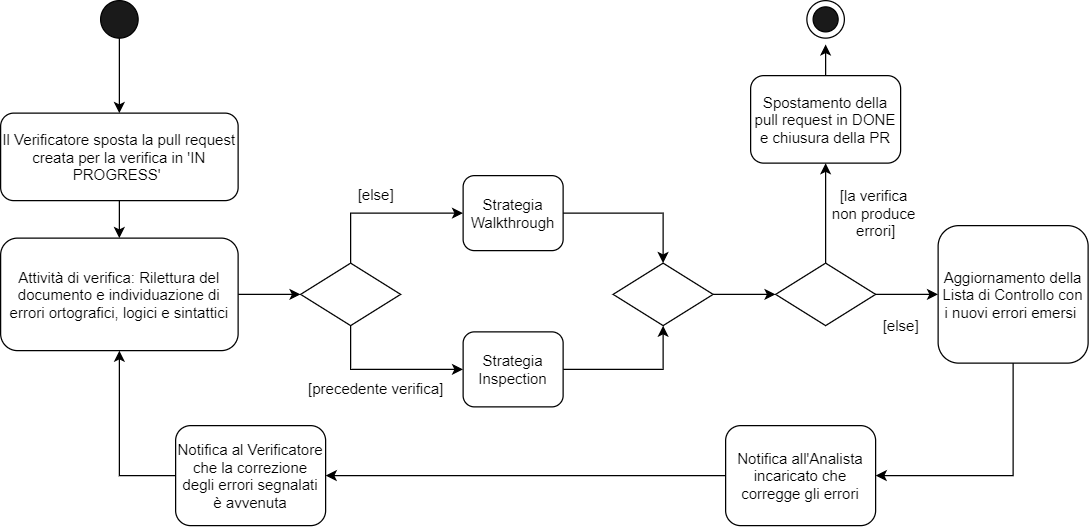
\includegraphics[width=\linewidth]{res/images/processo_verifica.png}
    \caption{Processo di verifica  dei documenti}
\end{figure}
Il processo di verifica viene gestito con il meccanismo delle pull request, una sorta di issue avanzata messa a disposizione da \textit{Github} descritto in dettaglio in \S\ref{_cicloVitaTicket}.

\subsubsection{Verifica del codice}
Il codice viene verificato con test automatici e con misurazioni quantificabili specificate all'interno del \dext{PianoDiQualifica\_1.0.0}. Il codice quindi deve obbedire a questi criteri:
\begin{itemize}
    \item deve essere corretto rispetto ai test definiti e alle metriche adottate per quantificare la sua qualità;
    \item deve derivare dai requisiti richiesti in \dext{AnalisiDeiRequisiti\_1.0.0}.
\end{itemize}

\paragraph{Analisi statica}
Anche per il codice, come per la documentazione, la prima fase di verifica sarà caratterizzata dall'analisi statica. %per gli strumenti si aspetta di iniziare a fare codice

\paragraph{Analisi dinamica}
L'analisi dinamica prevede la verifica del codice mirata a rilevare gli errori mentre questo è in fase di esecuzione.  Questa fase è caratterizzata dall'esecuzione di una batteria di test per verificare il corretto funzionamento del codice prodotto.\\
Ogni test eseguito deve essere:
\begin{itemize}
    \item \textbf{decidibile}: sempre in grado di terminare restituendo un feedback binario (riuscito/ fallito);
    \item \textbf{ripetibile}: dato un certo input e delle precondizioni fissate, deve produrre sempre lo stesso output per ogni prova effettuata.
\end{itemize}
Ogni test presenta i seguenti parametri:
\begin{itemize}
    \item \textbf{Ambiente}: caratteristiche hardware e software sulle quali viene eseguito il test;
    \item \textbf{Stato iniziale}: lo stato del software al momento dell'avvio del test;
    \item \textbf{Input}: dati in ingresso inseriti;
    \item \textbf{Output}: dati in uscita attesi;
    \item \textbf{Ulteriori istruzioni}: ulteriori informazioni sulla configurazione iniziale, sull'interpretazione dei risultati ottenuti e sugli eventuali effetti collaterali che l'esecuzione può produrre.
\end{itemize}
Per il formato di output di un test è da preferirsi un file di log che esponga in maniera chiara e immediata i risultati.

\subsubsection{Verifica dei requisiti}
Anche i requisiti sono sottoposti al processo di verifica. Perché la verifica dia esito positivo è necessario che essi:

\begin{itemize}
    \item siano coerenti con la loro implementazione;
    \item abbiano un grado di complessità adeguato rispetto al tempo e alle risorse pianificate per la riuscita del progetto;
    \item si dimostrino verificabili e quantificabili;
    \item siano coerenti con gli accordi presi con il proponente, riportati all'interno del documento \\\dext{AnalisiDeiRequisiti\_1.0.0}.
\end{itemize}

\paragraph{Analisi statica}
I requisiti devono rispettare le proprietà di:
\begin{itemize}
    \item \textbf{verificabilità}: un requisito deve essere misurabile oggettivamente;
    \item \textbf{codice univoco}: un requisito deve essere identificato da un codice, differente per ogni requisito, in accordo con quanto descritto in \S\ref{_classificazioneRequisiti};
    \item \textbf{atomicità}: un requisito non deve essere divisibile.
\end{itemize}

\subsubsection{Test}
I test costituiscono l'attività fondamentale dell'analisi dinamica: il loro utilizzo permette di individuare bug e di dimostrare che l'applicativo sviluppato è conforme rispetto a tutti i requisiti concordati nell'\dext{AnalisiDeiRequisiti\_1.0.0}.\\
Verranno implementati tipi di test descritti di seguito, ognuno con uno scopo diverso e con un oggetto di verifica differente.
\paragraph{Test di unità}
Consiste nel testare la partizione più piccola di software: l'unità. Il corretto funzionamento di ogni unità deve essere testato prima di procedere alla sua integrazione.
Verranno normati e implementati durante il processo di codifica.

\paragraph{Test di integrazione}
Necessari per testare che le diverse unità si interfaccino correttamente: questo tipo di test è eseguito in maniera ricorsiva: ogni volta che un gruppo di unità esegue in maniera corretta questo viene testato unendolo ad un altro gruppo di unità via via più grande fino ad arrivare al test di sistema.
Verranno normati e considerati nel processo di progettazione.

\paragraph{Test di sistema}
Dopo che tutte le unità sono state testate ed è stata testata la loro integrazione viene eseguito il test dell'intero sistema. In questa fase si verifica che tutte le componenti interagiscano nel modo atteso e che l'applicazione soddisfi ciò che è stato definito nell'\dext{AnalisiDeiRequisiti\_1.0.0}.
I test di sistema dell'applicazione EmporioLambda saranno implementati con \glock{Selenium} e sono stati definiti nel \dext{PianoDiQualifica\_1.0.0} durante il processo di analisi dei requisiti.

\paragraph{Test di regressione}
Quando una o più unità vengono modificate si esegue questa tipologia di test che serve per accertarsi che le funzionalità precedentemente implementate e testate non siano state danneggiate dai cambiamenti apportati al software.


\subsection{Validazione}
\label{_validazione}
\subsubsection{Scopo}
Questo processo assicura che il prodotto rispetti i requisiti e soddisfi le aspettative del proponente.

\subsubsection{Descrizione}
Per svolgere quanto sopra descritto si  usa come input l'output del processo di verifica,
restituendolo con la garanzia che soddisfi i requisiti.\\
Il principale attore è il \textit{Responsabile di Progetto}, il quale ha l'onere di decidere
se accettare e quindi approvare il prodotto oppure rigettarlo, indicando quali verifiche sono mancanti.

\subsubsection{Aspettative}
Per avviare il processo di validazione devono essere presenti questi elementi:
\begin{itemize}
    \item identificazione degli elementi da validare (documenti e/o codice sorgente);
    \item adottare una strategia di validazione che permetta di riutilizzare le procedure usate
          per la validazione;
    \item valutazione dei risultati rispetto alle attese.
\end{itemize}

\subsubsection{Validazione dei documenti}
\begin{figure}[h!]
    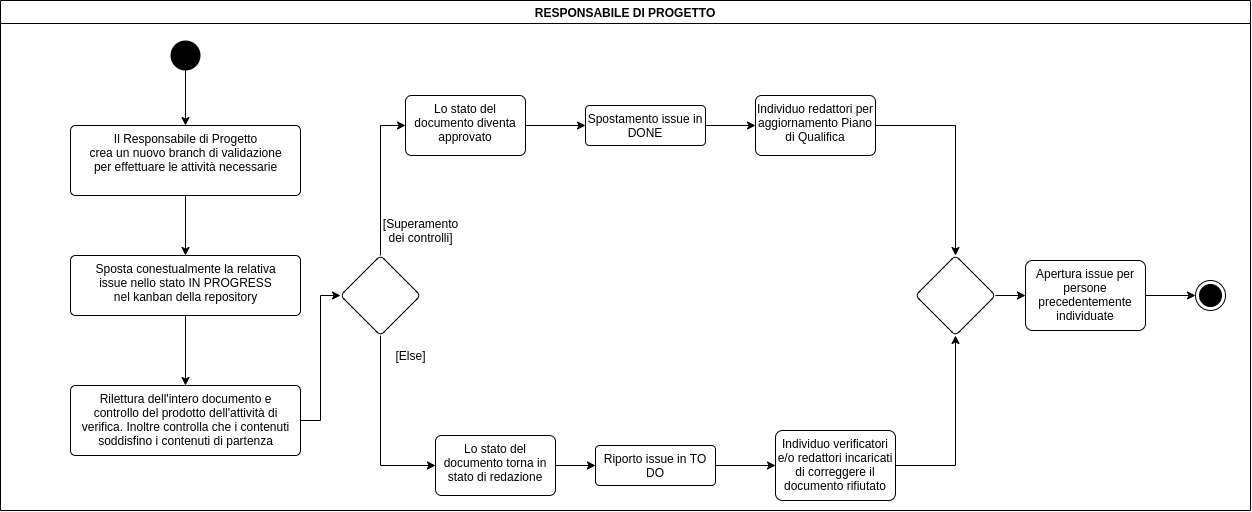
\includegraphics[width=\linewidth]{res/images/processo_validazione.png}
    \caption{Processo di validazione documenti}
\end{figure}

% \subsubsection{Attività per la validazione}

% \subsubsection{Test di validazione}

% \subsubsection{Responsabilità dei test}

% \paragraph{Codice identificativo dei test}
% Ogni test è descritto mediante:
% \begin{itemize}
%     \item codice identificativo:
%     \item descrizione;
%     \item stato, che può essere:
%     \begin{itemize}
%         \item implementato;
%         \item non implementato;
%         \item superato;
%         \item non superato.
%     \end{itemize}
% \end{itemize}
% Il codice identificativo si presenta nella seguente forma:
% \begin{center}
%     \textbf{T[Tipo][ID]}
% \end{center}
% dove:
% \begin{itemize}
%     \item \textbf{Tipo}: indica la tipologia del test e può assumere i valori:
%     \begin{itemize}
%         \item \textbf{U}: test di unità;
%         \item \textbf{I}: test di integrazione;
%         \item \textbf{S}: test di sistema;
%         \item \textbf{R}: test di regressione;
%         \item \textbf{V}: test di validazione.
%     \end{itemize}
%     \item \textbf{ID}: i valori che questo può assumere sono:
%     \begin{itemize}
%         \item \textbf{IDNumerico}: se si tratta di un test di unità, di integrazione o di regressione. Viene espresso con un numero progressivo;
%         \item \textbf{IDRequisito}: per i test di validazione e di sistema. È composto da:
%         \begin{center}
%             \textbf{[Tipo][Importanza][Codice]} 
%         \end{center}
%         secondo quanto descritto in \S\ref{_processoAnalisiDeiRequisiti} e indica il codice del requisito.
%     \end{itemize}
% \end{itemize}
